\documentclass[aspectratio=169,10pt]{beamer}

\usepackage[utf8]{inputenc}
\usepackage[T1]{fontenc}

\usetheme{Madrid}
\usecolortheme{seahorse}

\usepackage{amsmath}
\usepackage{amssymb}
\usepackage{amsfonts}
\usepackage{mathtools}
\usepackage{graphicx}
\usepackage{listings}
\usepackage{xcolor}
\usepackage{array}
\usepackage{booktabs}

\graphicspath{{figures/}}

% Code listing style
\lstset{
  basicstyle=\ttfamily\scriptsize,
  numbers=left,
  numberstyle=\tiny,
  stepnumber=1,
  numbersep=5pt,
  frame=single,
  breaklines=true,
  keywordstyle=\color{blue},
  commentstyle=\color{green!50!black}\itshape,
  stringstyle=\color{red},
  showstringspaces=false,
  language=Python
}

\setbeamertemplate{footline}[frame number]
\setbeamertemplate{navigation symbols}{}

\title{Weakly Contractive Mappings and Fixed Point Theorems}
\subtitle{Pathak: An Introduction to Nonlinear Analysis and Fixed Point Theory (Ch.~5, \S5.1)}
\author{Lecture Notes}
\date{2024}

\begin{document}

\frame{\titlepage}

\begin{frame}{Outline}
  \tableofcontents
\end{frame}

% ============================================================================
\section{Introduction: Classical Fixed Point Theorems}
% ============================================================================

\begin{frame}{Fixed Point Theorem: Classical Formulation}
  \begin{definition}[Fixed Point]
    Let $T : X \to X$ be a mapping. An element $u \in X$ is called a fixed point of $T$ if
    \[
      T(u) = u.
    \]
  \end{definition}

  \vspace{0.3cm}

  \begin{theorem}[Banach Contraction Mapping Principle]
    Let $(X, d)$ be a complete metric space and $T : X \to X$ a mapping such that there
    exists $\lambda \in [0,1)$ with
    \[
      d(Tx, Ty) \leq \lambda \, d(x,y) \quad \forall x, y \in X.
    \]
    Then:
    \begin{enumerate}
      \item $T$ has a unique fixed point $u \in X$;
      \item For any $x_0 \in X$, the sequence $\{T^n(x_0)\}$ converges to $u$;
      \item $d(T^n(x_0), u) \leq \frac{\lambda^n}{1-\lambda} d(x_0, T(x_0))$.
    \end{enumerate}
  \end{theorem}
\end{frame}

\begin{frame}{Illustration: Contraction Mapping Principle}
  \begin{center}
    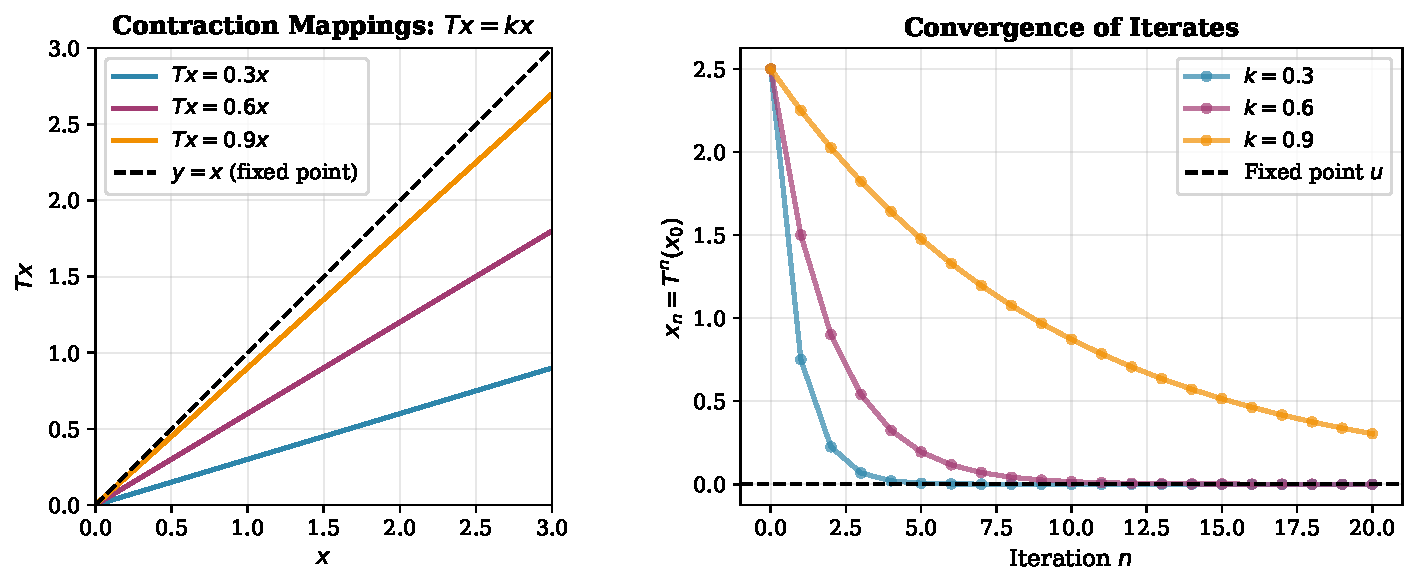
\includegraphics[width=0.95\textwidth]{fig_contraction_mapping_principle.pdf}
  \end{center}
  \small
  \textbf{Left:} Different contraction constants $k = 0.3, 0.6, 0.9$ show how smaller
  constants yield steeper contractions.
  \textbf{Right:} Convergence rates of iterates $x_n = T^n(x_0)$ depend on the contraction constant.
\end{frame}

% ============================================================================
\section{Kannan and Chatterjea Contractions}
% ============================================================================

\begin{frame}{Kannan's Contraction}
  \begin{theorem}[Kannan, 1968]
    Let $(X, d)$ be a complete metric space and $T : X \to X$ such that there exists
    $r \in [0, \tfrac{1}{2})$ with
    \[
      d(Tx, Ty) \leq r[d(Tx, y) + d(Ty, x)] \quad \text{(KC)}
    \]
    for all $x, y \in X$. Then $T$ has a unique fixed point $u \in X$.
  \end{theorem}

  \vspace{0.3cm}

  \textbf{Key Observation:} Kannan's condition involves \emph{mixed distances}:
  \begin{itemize}
    \item $d(Tx, y)$: distance from image of $x$ to $y$
    \item $d(Ty, x)$: distance from image of $y$ to $x$
  \end{itemize}

  \vspace{0.3cm}

  \textbf{Advantage:} $T$ need not be continuous at the fixed point.

  \vspace{0.3cm}

  \textbf{Example:} For $X = \mathbb{R}$ with usual metric, define
  \[
    T(x) = \begin{cases} 0 & \text{if } x \in (-\infty, 2], \\ \frac{1}{2} & \text{if } x \in (2, +\infty). \end{cases}
  \]
  Then $T$ satisfies Kannan's contraction with $r = \tfrac{1}{5}$ but is discontinuous at $x=2$.
\end{frame}

\begin{frame}{Chatterjea's Contraction}
  \begin{theorem}[Chatterjea, 1972]
    Let $(X, d)$ be a complete metric space and $T : X \to X$ such that there exists
    $r \in [0, \tfrac{1}{2})$ with
    \[
      d(Tx, Ty) \leq r[d(Tx, y) + d(Ty, x)] \quad \text{(CHC)}
    \]
    for all $x, y \in X$. Then $T$ has a unique fixed point $u \in X$.
  \end{theorem}

  \vspace{0.3cm}

  \textbf{Remark:} Chatterjea's condition has the same form as Kannan's! The \emph{difference}
  lies in the interpretation and context of application.

  \vspace{0.3cm}

  \begin{theorem}[Rhoades, 1977]
    The contractive conditions:
    \begin{itemize}
      \item Banach's contraction (BC)
      \item Kannan's contraction (KC)
      \item Chatterjea's contraction (CHC)
    \end{itemize}
    are \textbf{independent}, i.e., none implies the others in general.
  \end{theorem}
\end{frame}

\begin{frame}{Geometric Comparison: Kannan and Chatterjea}
  \begin{center}
    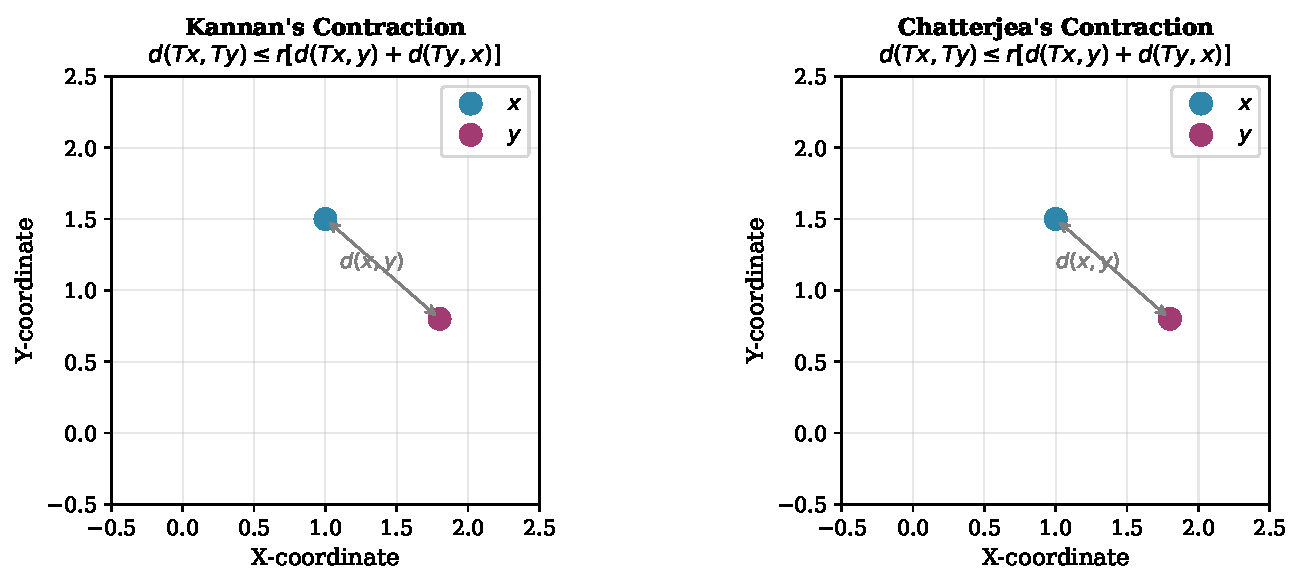
\includegraphics[width=0.9\textwidth]{fig_kannan_chatterjea.pdf}
  \end{center}
  \small
  Both contractions use mixed distance terms. Kannan's and Chatterjea's conditions
  relax the requirement of linearity found in Banach contractions, allowing
  non-continuous mappings to have fixed points.
\end{frame}

% ============================================================================
\section{Meir-Keeler and Reich Contractions}
% ============================================================================

\begin{frame}{Meir-Keeler Contraction}
  \begin{theorem}[Meir-Keeler, 1969]
    Let $(X, d)$ be a complete metric space and $T : X \to X$ such that for every
    $\varepsilon > 0$ there exists $\delta > 0$ with
    \[
      \varepsilon \leq d(x,y) < \varepsilon + \delta \implies d(Tx, Ty) < \varepsilon \quad \text{(MK)}
    \]
    Then $T$ is \emph{contractive}, i.e., $d(Tx, Ty) < d(x,y)$ for all $x \neq y$.
  \end{theorem}

  \vspace{0.3cm}

  \textbf{Consequence:} If $T$ is contractive and $(X,d)$ is complete, then $T$ has a unique
  fixed point.

  \vspace{0.3cm}

  \textbf{Key Property:} Meir-Keeler contractions are \emph{contractive} (strict inequality)
  but need not be Lipschitz contractions (no linear constant $\lambda$).

  \vspace{0.3cm}

  \textbf{Interpretation:} For any positive distance threshold $\varepsilon$, there exists
  a ``band'' of widths $\delta$ such that distances in this band are reduced below $\varepsilon$.
\end{frame}

\begin{frame}{Reich Contraction}
  \begin{theorem}[Reich, 1971]
    Let $(X, d)$ be a complete metric space and $T : X \to X$ such that there exist
    $a, b, c \in [0,1)$ with $a + b + c < 1$ and
    \[
      d(Tx, Ty) \leq a \, d(x,y) + b \, d(x, Tx) + c \, d(y, Ty) \quad \text{(RC)}
    \]
    for all $x, y \in X$. Then $T$ has a unique fixed point $u \in X$.
  \end{theorem}

  \vspace{0.3cm}

  \textbf{Generalization:} Reich's condition combines:
  \begin{itemize}
    \item Distance between $x$ and $y$ (Banach-type term)
    \item Orbit information: distances $d(x, Tx)$ and $d(y, Ty)$
  \end{itemize}

  \vspace{0.3cm}

  \textbf{Parameter Space:} The feasible region is $\{(a,b,c) : a,b,c \geq 0, \, a+b+c < 1\}$.
\end{frame}

\begin{frame}{Comparison: Meir-Keeler and Reich}
  \begin{center}
    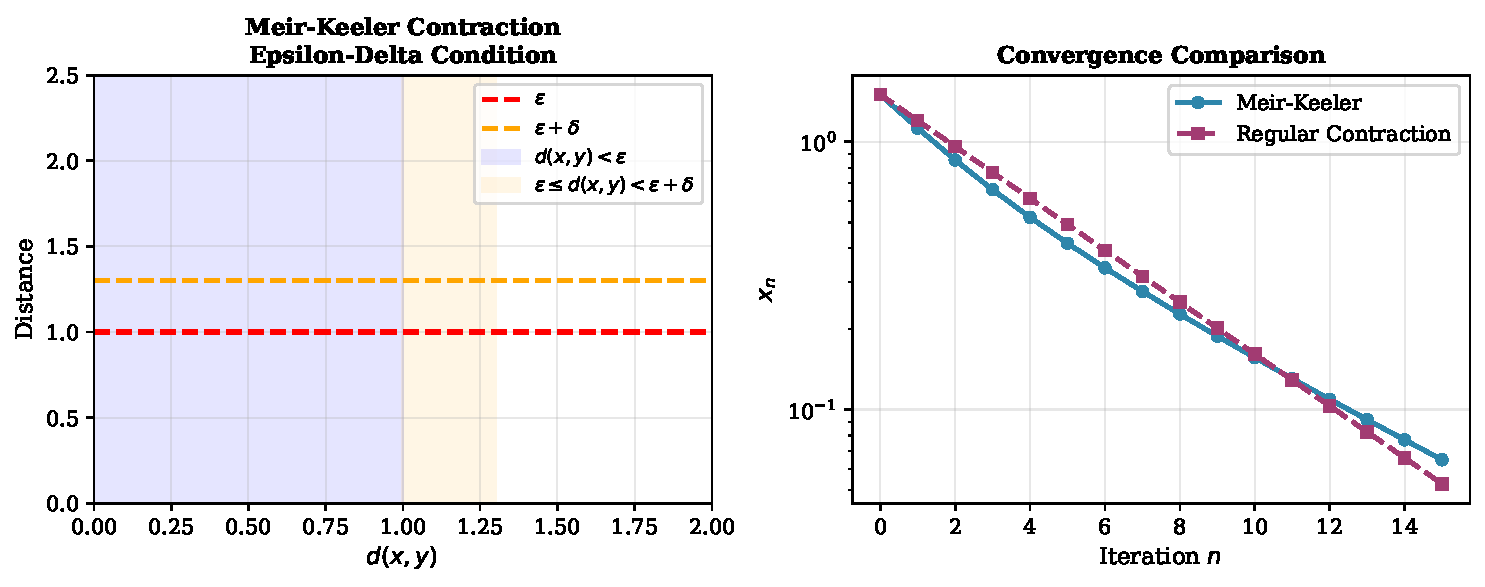
\includegraphics[width=0.95\textwidth]{fig_meir_keeler.pdf}
  \end{center}
  \small
  \textbf{Left:} Meir-Keeler's epsilon-delta condition creates flexible contraction behavior.
  \textbf{Right:} Convergence comparison shows how different contraction types affect
  the rate of convergence (note log scale).
\end{frame}

% ============================================================================
\section{Čirić and Hardy-Rogers Contractions}
% ============================================================================

\begin{frame}{Čirić Contraction}
  \begin{theorem}[Čirić, 1971]
    Let $(X, d)$ be a complete metric space and $T : X \to X$ such that there exist
    $a, b, c, e \in [0,1)$ with $a + b + c + 2e < 1$ and
    \[
      d(Tx, Ty) \leq a \, d(x,y) + b \, d(x, Tx) + c \, d(y, Ty) + e[d(x, Ty) + d(y, Tx)]
    \]
    for all $x, y \in X$. Then $T$ has a unique fixed point $u \in X$.
  \end{theorem}

  \vspace{0.3cm}

  \textbf{Generalization:} Čirić adds two new terms:
  \begin{itemize}
    \item $d(x, Ty)$: mixed distance from $x$ to image of $y$
    \item $d(y, Tx)$: mixed distance from $y$ to image of $x$
  \end{itemize}

  \vspace{0.3cm}

  \textbf{Strictest Condition:} The constraint $a + b + c + 2e < 1$ is the most restrictive
  among the contractions discussed so far.
\end{frame}

\begin{frame}{Hardy-Rogers Contraction}
  \begin{theorem}[Hardy-Rogers, 1973]
    Let $(X, d)$ be a complete metric space and $T : X \to X$ such that there exist
    $a_1, a_2, a_3, a_4, a_5 \in [0,1)$ with $\sum_{j=1}^5 a_j < 1$ and
    \[
      \begin{aligned}
        d(Tx, Ty) \leq & a_1 \, d(x, Tx) + a_2 \, d(y, Ty) + a_3 \, d(x, Ty) \\
                        & + a_4 \, d(y, Tx) + a_5 \, d(x,y)
      \end{aligned}
    \]
    for all $x, y \in X$. Then $T$ has a unique fixed point $u \in X$.
  \end{theorem}

  \vspace{0.3cm}

  \textbf{Most General:} Five independent parameters allow maximum flexibility in defining
  the contraction behavior.
\end{frame}

\begin{frame}{Čirić and Hardy-Rogers Comparison}
  \begin{center}
    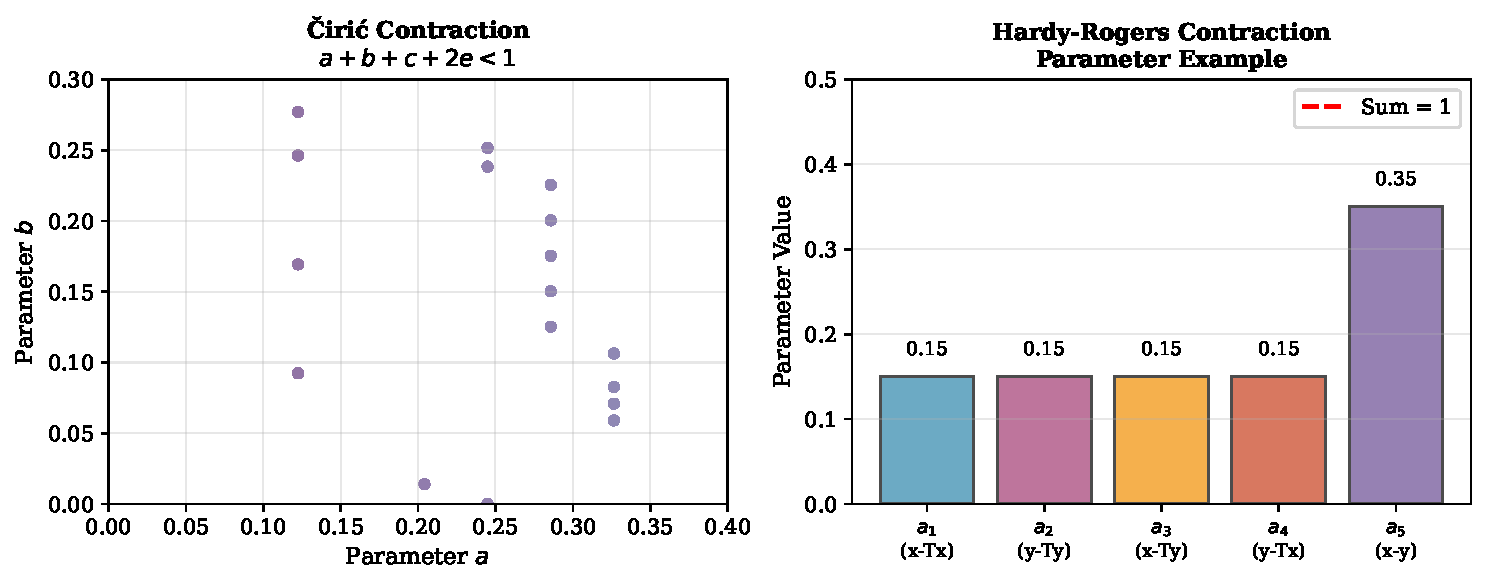
\includegraphics[width=0.95\textwidth]{fig_ciric_hardy_rogers.pdf}
  \end{center}
  \small
  \textbf{Left:} Parameter space for Čirić contractions showing feasible regions.
  \textbf{Right:} Example of Hardy-Rogers parameter values. The constraint
  $\sum a_i < 1$ ensures convergence while allowing flexible weighting of different distance measures.
\end{frame}

% ============================================================================
\section{Specialized Cases: Zamfirescu and Berinde}
% ============================================================================

\begin{frame}{Zamfirescu Contraction}
  \begin{theorem}[Zamfirescu, 1972]
    Let $(X, d)$ be a complete metric space and $T : X \to X$ such that
    \[
      d(Tx, Ty) \leq \max\left\{d(x,y), \tfrac{1}{2}[d(x, Tx) + d(y, Ty)], \tfrac{1}{2}[d(x, Ty) + d(y, Tx)]\right\}
    \]
    for all $x, y \in X$. Then $T$ has a unique fixed point $u \in X$.
  \end{theorem}

  \vspace{0.3cm}

  \textbf{Key Feature:} Uses \emph{maximum} of three distance expressions, providing a
  non-linear contractive condition.

  \vspace{0.3cm}

  \textbf{Flexibility:} The mapping contracts relative to whichever distance measure is
  largest, allowing asymmetric behavior.
\end{frame}

\begin{frame}{Berinde Contraction}
  \begin{theorem}[Berinde, 2004]
    Let $(X, d)$ be a complete metric space and $T : X \to X$ such that there exist
    $r \in [0,1)$ and $L \geq 0$ with
    \[
      d(Tx, Ty) \leq r \, d(x,y) + L \, d(y, Tx)
    \]
    for all $x, y \in X$. Then $T$ has a unique fixed point $u \in X$.
  \end{theorem}

  \vspace{0.3cm}

  \textbf{Quasi-contraction:} Berinde's condition involves both:
  \begin{itemize}
    \item A standard contraction term: $r \, d(x,y)$
    \item An auxiliary term: $L \, d(y, Tx)$
  \end{itemize}

  \vspace{0.3cm}

  \textbf{Application:} Useful in cases where the linear term alone does not guarantee contraction.
\end{frame}

% ============================================================================
\section{Converse of Banach Contraction Principle}
% ============================================================================

\begin{frame}{Bessaga's Converse Theorem}
  \begin{theorem}[Bessaga, 1959]
    Let $X$ be an arbitrary set and $T : X \to X$ such that $T^n$ has a unique fixed point
    $u \in X$ for every $n \geq 1$. Then for every $\lambda \in (0,1)$, there exists
    a metric $d = d_\lambda$ on $X$ such that:
    \begin{enumerate}
      \item $(X, d)$ is a complete metric space;
      \item $T$ is a contraction on $(X, d)$ with Lipschitz constant $\lambda$.
    \end{enumerate}
  \end{theorem}

  \vspace{0.3cm}

  \textbf{Significance:} Shows that the Banach contraction principle is \emph{complete}
  --- having unique fixed points for all iterates is equivalent to the existence of
  a metric making $T$ a contraction.

  \vspace{0.3cm}

  \textbf{Construction Key:}
  \begin{itemize}
    \item Partition $X$ into equivalence classes under the relation $T$
    \item Define distance $d(x, u) = \lambda^{-n}$ if $T^n(x) = u$
  \end{itemize}
\end{frame}

\begin{frame}{Illustration: Bessaga's Converse}
  \begin{center}
    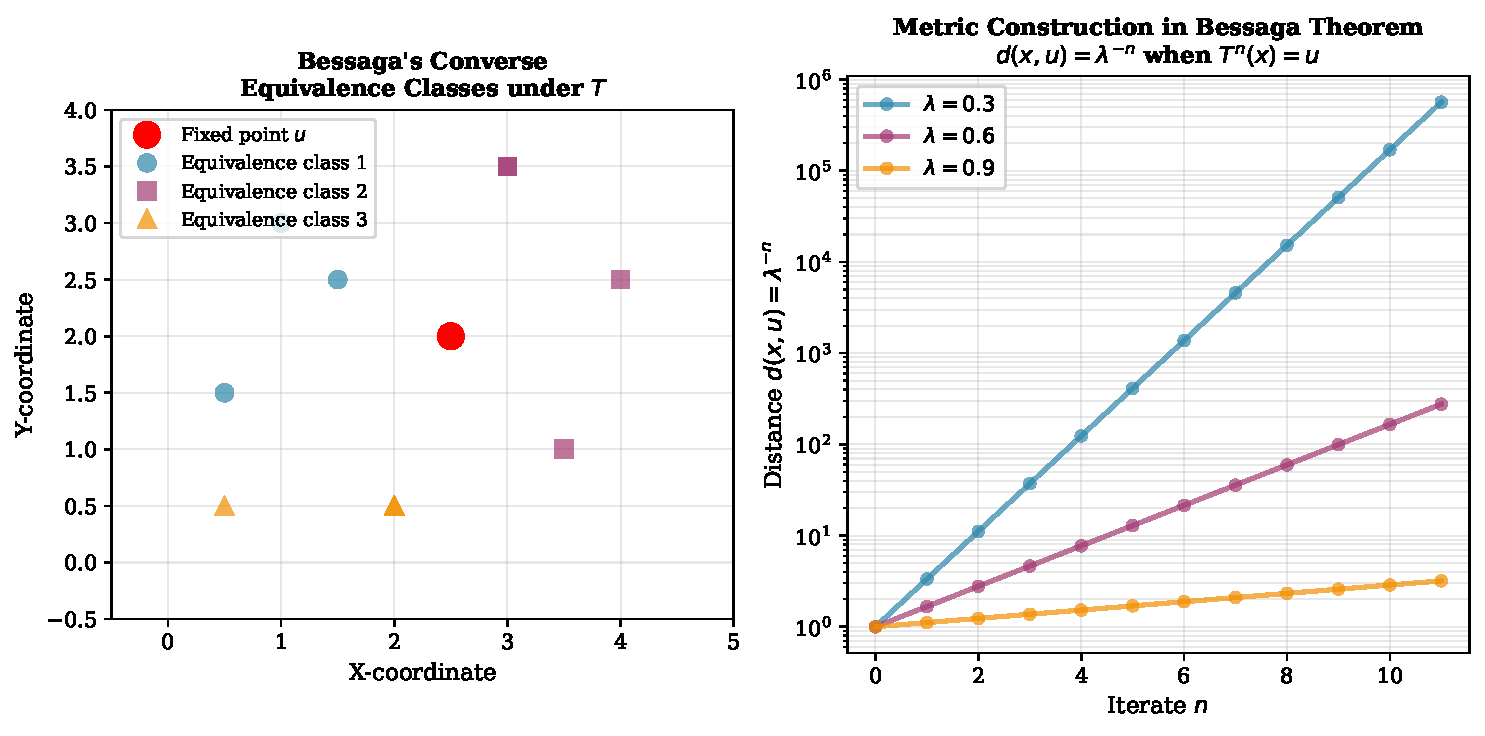
\includegraphics[width=0.95\textwidth]{fig_bessaga_theorem.pdf}
  \end{center}
  \small
  \textbf{Left:} Equivalence classes under the action of $T$ partition the space.
  Each class has points related by iteration.
  \textbf{Right:} The constructed metric $d(x,u) = \lambda^{-n}$ (when $T^n(x) = u$)
  grows exponentially with the number of iterations needed to reach the fixed point.
\end{frame}

% ============================================================================
\section{(\varepsilon ,k)-Uniformly Locally Contractive Mappings}
% ============================================================================

\begin{frame}{\varepsilon -Chainable Metric Spaces}
  \begin{definition}[\varepsilon -Chain]
    Let $(X,d)$ be a metric space and $\varepsilon > 0$. A finite sequence
    $x_0, x_1, \ldots, x_n$ of points in $X$ is called an $\varepsilon$-chain joining
    $x_0$ and $x_n$ if
    \[
      d(x_{i-1}, x_i) < \varepsilon \quad \text{for } i = 1, 2, \ldots, n.
    \]
    The metric space $(X,d)$ is \emph{$\varepsilon$-chainable} if for each pair $(x,y)$
    of its points, there exists an $\varepsilon$-chain joining them.
  \end{definition}

  \vspace{0.3cm}

  \textbf{Interpretation:} The space can be connected by chains of small steps of size less than $\varepsilon$.

  \vspace{0.3cm}

  \textbf{Examples:} Connected metric spaces (e.g., intervals in $\mathbb{R}$, connected
  subsets of $\mathbb{R}^n$).
\end{frame}

\begin{frame}{(\varepsilon ,k)-Uniformly Locally Contractive Mappings}
  \begin{definition}
    A mapping $T : X \to X$ is called $(\varepsilon, k)$-uniformly locally contractive
    if there exists $\varepsilon > 0$ and $k \in [0,1)$ such that
    \[
      d(x,y) < \varepsilon \implies d(Tx, Ty) \leq k \, d(x,y) \quad \text{for all } x,y \in X.
    \]
  \end{definition}

  \vspace{0.3cm}

  \textbf{Key Property:} $T$ contracts distances only when they are below the threshold $\varepsilon$.

  \vspace{0.3cm}

  \textbf{Comparison:}
  \begin{itemize}
    \item \textbf{Standard Contraction:} Contracts all distances
    \item \textbf{Locally Contractive:} Contracts only small distances
  \end{itemize}
\end{frame}

\begin{frame}{Edelstein Theorem}
  \begin{theorem}[Edelstein, 1962]
    Let $(X, d)$ be a complete $\varepsilon$-chainable metric space and $T : X \to X$
    be an $(\varepsilon, k)$-uniformly locally contractive mapping. Then:
    \begin{enumerate}
      \item $T$ has a unique fixed point $u \in X$;
      \item For any $x_0 \in X$, the sequence $\{T^n x_0\}$ converges to $u$.
    \end{enumerate}
  \end{theorem}

  \vspace{0.3cm}

  \textbf{Proof Idea:}
  \begin{enumerate}
    \item Define a new metric $d_\varepsilon(x,y) = \inf \sum d(x_{i-1}, x_i)$ over all
      $\varepsilon$-chains
    \item Show that $T$ is a contraction with respect to $d_\varepsilon$
    \item Apply Banach fixed point theorem
  \end{enumerate}

  \vspace{0.3cm}

  \textbf{Significance:} Generalizes contraction principle to spaces that are only
  locally contractive rather than globally contractive.
\end{frame}

\begin{frame}{Illustration: \varepsilon -Chainable Spaces and Edelstein}
  \begin{center}
    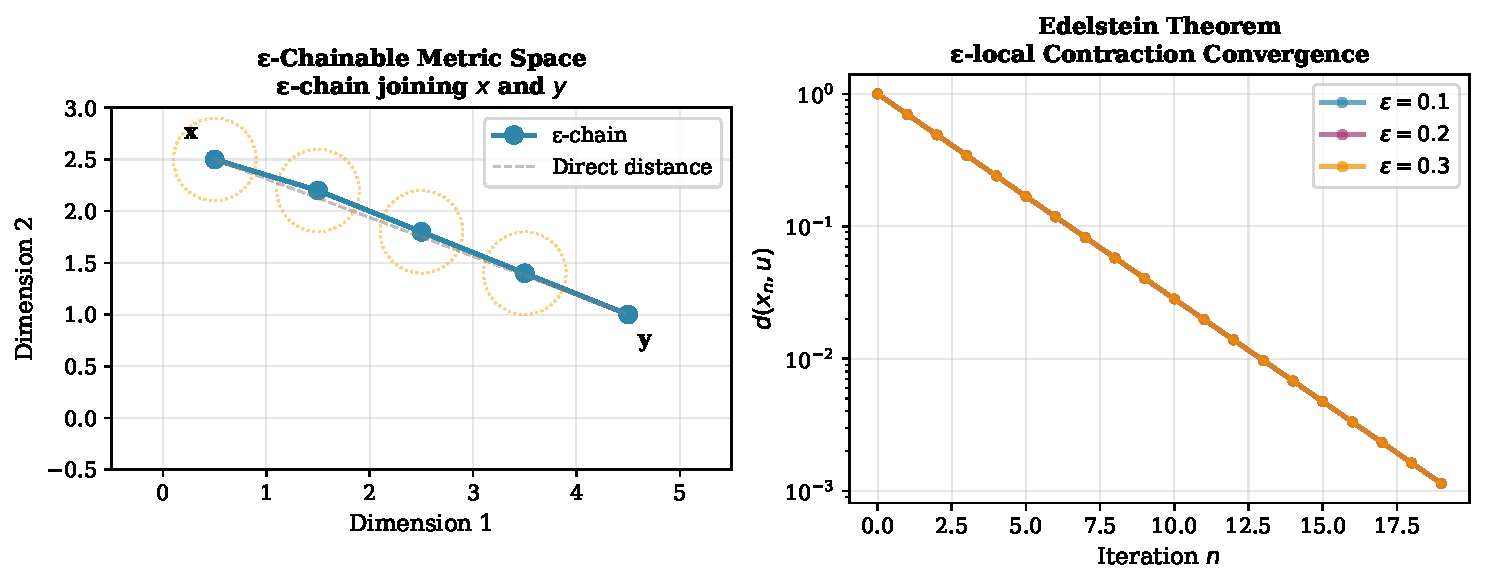
\includegraphics[width=0.95\textwidth]{fig_epsilon_chainable_spaces.pdf}
  \end{center}
  \small
  \textbf{Left:} An \varepsilon -chain connects distant points through intermediate steps.
  \textbf{Right:} Convergence under locally contractive mappings with different
  \varepsilon -localization parameters.
\end{frame}

% ============================================================================
\section{Generalized Contractions: Summary and Hierarchy}
% ============================================================================

\begin{frame}{Hierarchy of Contractive Mappings}
  \begin{center}
    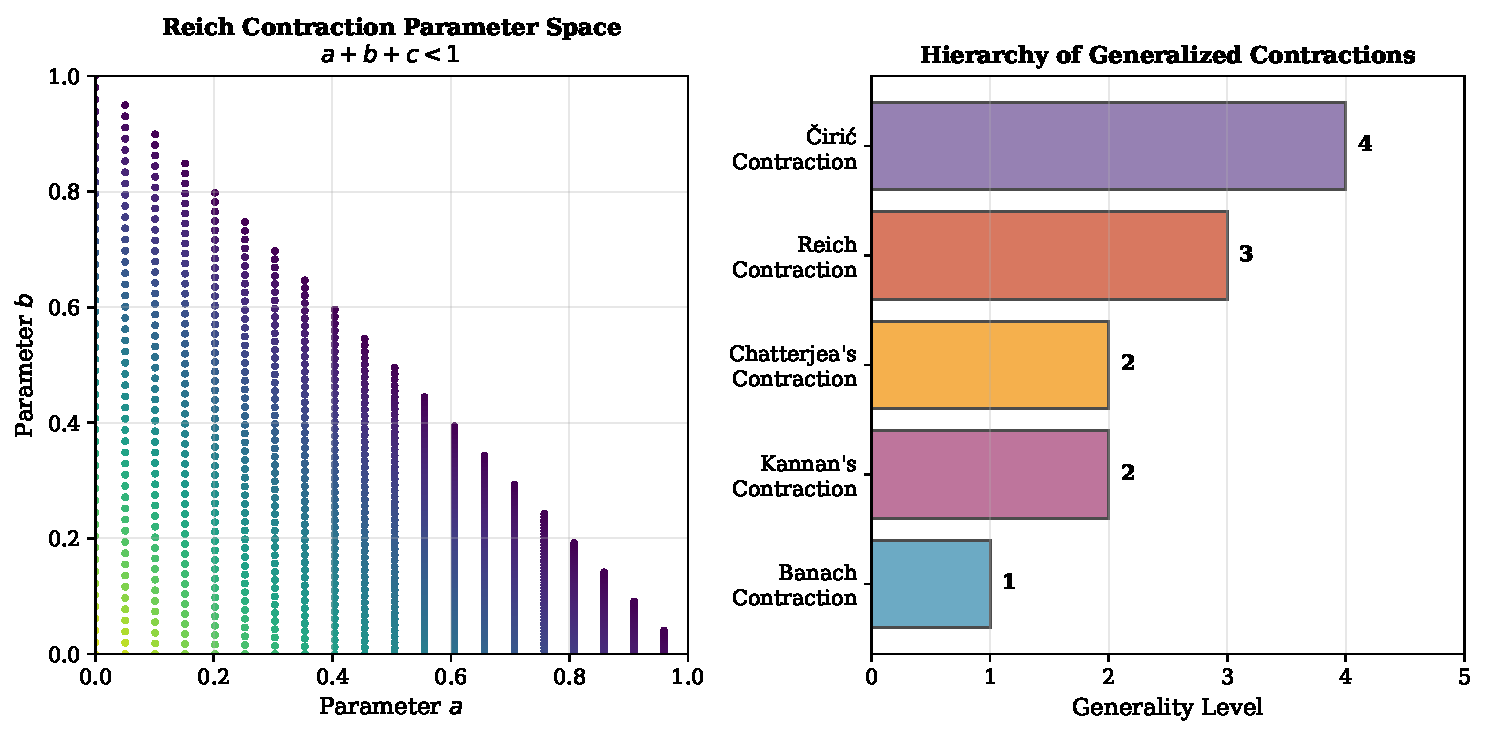
\includegraphics[width=0.9\textwidth]{fig_reich_contraction.pdf}
  \end{center}
  \small
  Different contraction types form a hierarchy of generality. More general conditions
  allow weaker assumptions on the mapping $T$ while still guaranteeing a unique fixed point.
\end{frame}

\begin{frame}{Summary: Generalized Contraction Types}
  \begin{table}
    \centering
    \small
    \begin{tabular}{lll}
      \toprule
      \textbf{Type} & \textbf{Condition} & \textbf{Year} \\
      \midrule
      Banach & $d(Tx,Ty) \leq \lambda d(x,y)$ & 1922 \\
      Kannan & $d(Tx,Ty) \leq r[d(Tx,y) + d(Ty,x)]$, $r < 1/2$ & 1968 \\
      Chatterjea & $d(Tx,Ty) \leq r[d(Tx,y) + d(Ty,x)]$, $r < 1/2$ & 1972 \\
      Meir-Keeler & $\varepsilon \leq d(x,y) < \varepsilon+\delta \Rightarrow d(Tx,Ty) < \varepsilon$ & 1969 \\
      Reich & $d(Tx,Ty) \leq ad(x,y) + bd(x,Tx) + cd(y,Ty)$ & 1971 \\
      Čirić & Above + $e[d(x,Ty) + d(y,Tx)]$, $a+b+c+2e < 1$ & 1971 \\
      Hardy-Rogers & 5 parameters: $\sum a_i < 1$ & 1973 \\
      Zamfirescu & Max of three expressions & 1972 \\
      Berinde & $d(Tx,Ty) \leq rd(x,y) + Ld(y,Tx)$ & 2004 \\
      \bottomrule
    \end{tabular}
  \end{table}
\end{frame}

\begin{frame}[fragile]{Numerical Example: Contraction Comparison}
  \begin{lstlisting}
# Numerical comparison of convergence rates
import numpy as np

def iterate_T(x0, k, n_iter=20):
    """Simulate T^n(x0) = k*x0 converging to 0"""
    return [x0 * k**n for n in range(n_iter)]

# Compare different contraction constants
k_values = [0.3, 0.6, 0.9]
x0 = 1.0

for k in k_values:
    iterates = iterate_T(x0, k, 15)
    print(f"k = {k}:")
    for n, x_n in enumerate(iterates[:5]):
        print(f"  x_{n} = {x_n:.6f}")

    # Estimate order of convergence
    rates = [np.log(iterates[n+1]/iterates[n])
             for n in range(len(iterates)-1) if iterates[n] > 1e-10]
    print(f"  Convergence rate: {np.mean(rates):.4f}")
    print()
  \end{lstlisting}
\end{frame}

% ============================================================================
\section{Applications and Remarks}
% ============================================================================

\begin{frame}{Applications of Generalized Contractions}
  \begin{enumerate}
    \item \textbf{Differential Equations:} Many existence and uniqueness theorems for ODEs
      rely on contraction principles

    \vspace{0.2cm}

    \item \textbf{Integral Equations:} Fixed point methods solve Volterra and Fredholm equations

    \vspace{0.2cm}

    \item \textbf{Optimization:} Iterative methods for minimization use contractive principles

    \vspace{0.2cm}

    \item \textbf{Numerical Analysis:} Newton-Raphson and related methods use contraction
      properties

    \vspace{0.2cm}

    \item \textbf{Economics:} Equilibrium problems in game theory and markets

    \vspace{0.2cm}

    \item \textbf{Dynamical Systems:} Stability analysis and bifurcation theory
  \end{enumerate}
\end{frame}

\begin{frame}{Independence of Contraction Types}
  \begin{theorem}[Rhoades, 1977]
    The following contractive conditions are \textbf{independent}:
    \begin{itemize}
      \item Banach contraction (BC)
      \item Kannan contraction (KC)
      \item Chatterjea contraction (CHC)
    \end{itemize}
    meaning that none implies the others in general.
  \end{theorem}

  \vspace{0.3cm}

  \textbf{Implications:}
  \begin{itemize}
    \item Each contraction type captures different aspects of contractive behavior
    \item The choice of contraction depends on the problem structure
    \item Generality comes at the cost of more complex conditions
  \end{itemize}

  \vspace{0.3cm}

  \textbf{Open Question:} How can we systematically search for the ``right'' contraction
  type for a given problem?
\end{frame}

\begin{frame}{Key Theorems Summary}
  \begin{table}
    \centering
    \small
    \begin{tabular}{ll}
      \toprule
      \textbf{Theorem} & \textbf{Conclusion} \\
      \midrule
      Banach Contraction & Unique fixed point exists \\
      Kannan Fixed Point & Unique fixed point (non-continuous) \\
      Chatterjea Fixed Point & Unique fixed point (non-continuous) \\
      Meir-Keeler & Contractive implies unique fixed point \\
      Reich Fixed Point & Unique fixed point (mixed distances) \\
      Čirić Fixed Point & Unique fixed point (most general linear) \\
      Hardy-Rogers Fixed Point & Unique fixed point (5 parameters) \\
      Bessaga Converse & Metric can be constructed from iterates \\
      Edelstein Theorem & Unique fixed point in chainable spaces \\
      \bottomrule
    \end{tabular}
  \end{table}

  \vspace{0.3cm}

  \small
  \textbf{Common Theme:} All theorems guarantee existence of a unique fixed point
  under weaker contractive conditions than Banach's.
\end{frame}

% ============================================================================
\section{Recent Developments: Weakly Contractive Mappings}
% ============================================================================

\begin{frame}{Weakly Contractive Mappings (Banach Spaces)}
  \begin{definition}[Weakly Contractive Mapping - Banach Space]
    Let $X$ be a Banach space. A self-map $T : X \to X$ is \emph{weakly contractive} if
    for every $x, y \in X$,
    \[
      \|Tx - Ty\| \leq \|x - y\| - \psi(\|x - y\|),
    \]
    where $\psi : [0,\infty) \to [0,\infty)$ is continuous, nondecreasing, and satisfies:
    \begin{enumerate}
      \item $\psi(0) = 0$;
      \item $\psi(t) > 0$ for $t > 0$;
      \item $\lim_{t \to \infty} \psi(t) = \infty$.
    \end{enumerate}
  \end{definition}

  \vspace{0.2cm}

  \textbf{Examples of } $\psi$\textbf{:}
  \begin{itemize}
    \item $\psi(t) = at$ for $a \in (0,1)$ (linear)
    \item $\psi(t) = \frac{t^2}{t+1}$ (nonlinear)
    \item $\psi(t) = \ln(t+1)$ (logarithmic)
  \end{itemize}
\end{frame}

\begin{frame}{Weakly Contractive Mappings (Metric Spaces)}
  \begin{definition}[Weakly Contractive Mapping - Metric Space]
    Let $(X, d)$ be a metric space. A self-map $f : X \to X$ is \emph{weakly contractive}
    if for all $x, y \in X$,
    \[
      d(fx, fy) \leq d(x,y) - \psi(d(x,y))
    \]
    where $\psi$ satisfies the conditions above.
  \end{definition}

  \vspace{0.3cm}

  \textbf{Key Difference from Banach:}
  \begin{itemize}
    \item Weakly contractive: $d(fx,fy) \leq d(x,y) - \psi(d(x,y))$ (strict improvement)
    \item Contractive: $d(Tx,Ty) \leq \lambda d(x,y)$ with $\lambda < 1$ (linear ratio)
  \end{itemize}

  \vspace{0.3cm}

  \textbf{Advantage:} The decay function $\psi$ can be arbitrary (not necessarily linear),
  providing much flexibility.
\end{frame}

\begin{frame}{Theorems for Weakly Contractive Mappings}
  \begin{theorem}[Alber-Guerre-Delabriere]
    Let $(X, d)$ be a complete metric space and $f : X \to X$ be a weakly contractive map.
    Then $f$ has a unique fixed point $u \in X$.
  \end{theorem}

  \vspace{0.3cm}

  \begin{theorem}[Harjani-Sadarangani, 2009]
    Let $(X, \leq)$ be a partially ordered set with a metric $d$ such that $(X,d)$ is complete.
    Let $f : X \to X$ be continuous and nondecreasing such that
    \[
      d(fx, fy) \leq d(x,y) - \psi(d(x,y)) \quad \text{for } x \geq y
    \]
    If there exists $x_0 \in X$ with $x_0 \leq f(x_0)$, then $f$ has a fixed point.
  \end{theorem}

  \vspace{0.3cm}

  \textbf{Extension:} Weakly contractive mappings can be combined with ordering structures
  to handle more complex spaces.
\end{frame}

% ============================================================================
\section{Conclusion}
% ============================================================================

\begin{frame}{Summary and Main Takeaways}
  \begin{enumerate}
    \item \textbf{Classical Contraction:} Banach's principle requires global Lipschitz property

    \vspace{0.2cm}

    \item \textbf{Generalized Contractions:} Kannan, Chatterjea, Reich, Čirić, Hardy-Rogers
      progressively generalize the contraction condition

    \vspace{0.2cm}

    \item \textbf{Local Contractions:} Meir-Keeler and Edelstein theorems handle locally
      contractive mappings

    \vspace{0.2cm}

    \item \textbf{Converse Result:} Bessaga shows the principle is complete --- iterates
      determine the metric

    \vspace{0.2cm}

    \item \textbf{Modern Theory:} Weakly contractive mappings provide nonlinear decay
      guaranteeing convergence

    \vspace{0.2cm}

    \item \textbf{Applications:} These results apply to differential equations, integral equations,
      optimization, and dynamical systems
  \end{enumerate}
\end{frame}

\begin{frame}{Further Reading}
  \begin{itemize}
    \item Pathak, H. K. (2018). \textit{An Introduction to Nonlinear Analysis and Fixed Point Theory}.
      Springer.

    \vspace{0.3cm}

    \item Kirk, W. A., \& Sims, B. (Eds.). (2001). \textit{Handbook of Metric Fixed Point Theory}.
      Kluwer Academic Publishers.

    \vspace{0.3cm}

    \item Berinde, V. (2007). \textit{Iterative Approximation of Fixed Points}. Springer.

    \vspace{0.3cm}

    \item Khamsi, M. A., \& Kirk, W. A. (2011). \textit{An Introduction to Metric Spaces and
      Fixed Point Theory}. John Wiley \& Sons.
  \end{itemize}
\end{frame}

\begin{frame}[allowframebreaks]{Key Theorems at a Glance}
  \begin{itemize}
    \item \textbf{Banach (1922):} $d(Tx,Ty) \leq \lambda d(x,y)$ $\Rightarrow$ unique fixed point

    \item \textbf{Kannan (1968):} $d(Tx,Ty) \leq r[d(Tx,y) + d(Ty,x)]$, $r < 1/2$ $\Rightarrow$ unique fixed point

    \item \textbf{Chatterjea (1972):} Mixed-distance condition $\Rightarrow$ unique fixed point

    \item \textbf{Meir-Keeler (1969):} Epsilon-delta condition $\Rightarrow$ contractive $\Rightarrow$ unique fixed point

    \item \textbf{Reich (1971):} Linear combination of mixed distances $\Rightarrow$ unique fixed point

    \item \textbf{Čirić (1971):} Extends Reich with additional mixed terms

    \item \textbf{Hardy-Rogers (1973):} Five-parameter generalization

    \item \textbf{Rhoades (1977):} Basic contractions are independent

    \item \textbf{Bessaga (1959):} Metric construction from iterates

    \item \textbf{Edelstein (1962):} Local contractions in chainable spaces

    \item \textbf{Alber-Guerre-Delabriere:} Weakly contractive mappings

    \item \textbf{Harjani-Sadarangani (2009):} Weakly contractive in ordered spaces
  \end{itemize}
\end{frame}

\end{document}
